
\addchap{\textquotedblleft Applied functional type theory\textquotedblright :
A proposal\label{chap:Applied-functional-type}}

What exactly is the extent of \textsf{``}theory\textsf{''} that a software engineer
should know in order to be a proficient functional programmer? This
book proposes an answer to that question by presenting a coherent
body of theoretical knowledge that, in the author\textsf{'}s view, \emph{is}
the theory that underlies the practice of functional programming and
guides software engineers in writing code. This body of knowledge
may be viewed as a new emerging sub-branch of computer science, tentatively
called \textbf{\index{applied functional type theory}applied functional
type theory} (AFTT). 

In order to discover the proper scope of AFTT, this book appraises
the various inventions made in the field of functional programming
in the last 30 years, such as the \textquotedblleft functional pearls\textquotedblright{}
papers\footnote{\texttt{\href{https://wiki.haskell.org/Research_papers/Functional_pearls}{https://wiki.haskell.org/Research\_papers/Functional\_pearls}}}
and various online tutorials, looking for theoretical material that
has demonstrated its pragmatic usefulness. As a first step towards
formulating AFTT from the ground up, the results are presented in
the form of a tutorial, with motivations and rigorous derivations
of substantially all relevant mathematical facts.

In this book, code examples are written in Scala because the author
is fluent in that language. However, most of the material will work
equally well in Haskell, OCaml, and other FP languages. This is because
AFTT is the science of functional programming and not a set of tricks
specific to Scala or Haskell. An advanced user of any functional programming
language will have to face the same questions and struggle with the
same practical issues.

\addsec{AFTT is not covered by courses in computer science}

Traditional courses of computer science (algorithms and data structures,
complexity theory, distributed systems, databases, network systems,
compilers, operating systems) are largely not relevant to AFTT. Courses
in programming language theory are more relevant but are not presented
at an appropriate level. To an academic computer scientist, the theory
behind Haskell is \textsf{``}System $F\omega$\textsf{''}, a version of $\lambda$-calculus\index{System Fomega (Haskell)@System $F\omega$ (Haskell)}.\footnote{\texttt{\href{https://babel.ls.fi.upm.es/~pablo/Papers/Notes/f-fw.pdf}{https://babel.ls.fi.upm.es/$\sim$pablo/Papers/Notes/f-fw.pdf}}}
That theory guided the design of the Haskell language and defines
rigorously what a Haskell program means in a mathematical sense. The
theory behind Scala is called the \textsf{``}DOT\textsf{''} (dependent object type)
calculus.\footnote{\texttt{\href{https://www.scala-lang.org/blog/2016/02/03/essence-of-scala.html}{https://www.scala-lang.org/blog/2016/02/03/essence-of-scala.html}}}\index{dependent object type (DOT) calculus}
That theory guided the design of Scala version 3.

However, a practicing Haskell or Scala programmer is not concerned
with designing Haskell or Scala, or with proving theoretical properties
of those languages. Instead, the programmer is mainly concerned with
\emph{using} a chosen programming language to write code. 

Knowing how to prove various properties of System $F\omega$ or DOT
will not actually help programmers to write code. So, these theories
are outside the scope of AFTT. The practice of functional programming
does not require graduate-level theoretical studies.

As an example of theoretical material that \emph{is} within the scope
of AFTT, consider applicative functors (Chapter~\ref{chap:8-Applicative-functors,-contrafunctors}).\index{applicative functors}
It is helpful for a practicing functional programmer to be able to
recognize and use applicative functors. An applicative functor is
a data structure specifying declaratively some operations that can
run independently of each other. Programs may combine these operations,
execute them in parallel, check for validity, or refactor for optimization
or better maintainability.

To use this functionality, the programmer must begin by checking whether
a given data structure satisfies the laws of applicative functors.
In a given application, the choice of a data structure may be dictated
in part by the business logic. The programmer first writes down the
type of that data structure and the code implementing the required
methods. The programmer can then check whether the laws hold. The
data structure and the code may need to be adjusted in order to fit
the definition of an applicative functor and to make the laws hold.

So, the programmer needs to perform a certain amount of symbolic derivations
before coding. The derivations can be done using pen and paper by
writing equations in a concise mathematical notation. Once the laws
are verified, the programmer proceeds to write code.

The mathematical proofs and derivations assure that the chosen data
structure will satisfy the laws of applicative functors, no matter
how the rest of the program is written. So, for example, it is assured
that the relevant operations can be automatically parallelized and
will still work correctly. In this way, AFTT directly guides the programmer
and helps write correct code.

Applicative functors were discovered by practitioners who were using
Haskell to implement parser combinators for compilers. However, applicative
functors are not a feature of Haskell. Rather, they are a design pattern
that may be used in Scala or in any other functional programming language.
A prominent example of an applicative functor is Apache Spark\textsf{'}s \lstinline!RDD!
data type, which is widely used for implementing large-scale parallel
computations.\footnote{\texttt{\href{https://spark.apache.org/docs/latest/rdd-programming-guide.html}{https://spark.apache.org/docs/latest/rdd-programming-guide.html}}}
And yet, no standard computer science course or textbook defines applicative
functors, motivates their laws, explores their structure on examples,
or shows data types that are \emph{not} applicative functors (and
explains why not). 

\addsec{AFTT is not category theory, type theory, or formal logic}

One often hears that functional programming is based on category theory.\footnote{\texttt{\href{https://www.47deg.com/blog/science-behind-functional-programming/}{https://www.47deg.com/blog/science-behind-functional-programming/}}}
Indeed, the material shown in this book includes a (small) number
of notions from category theory, as well as from formal logic and
type theory. However, software engineers would not benefit from traditional
academic courses in those subjects: their presentation is too abstract
and at the same time lacks specific results necessary for practical
programming. Those courses answer questions that academic mathematicians
have, not questions that practicing functional programmers have.

There exist books intended as presentations of category theory for
computer scientists\footnote{See, e.g., \texttt{\href{https://www.amazon.com/dp/0262660717}{https://www.amazon.com/dp/0262660717}}
or \texttt{\href{https://www.math.mcgill.ca/triples/Barr-Wells-ctcs.pdf}{https://www.math.mcgill.ca/triples/Barr-Wells-ctcs.pdf}}} or for programmers.\footnote{\texttt{\href{https://github.com/hmemcpy/milewski-ctfp-pdf}{https://github.com/hmemcpy/milewski-ctfp-pdf}}}
However, those books do not cover certain concepts relevant to programming,
such as applicative\footnote{Applicative functors are known in mathematics as \textsf{``}monoidal\textsf{''}: \texttt{\href{https://en.wikipedia.org/wiki/Monoidal_functor}{https://en.wikipedia.org/wiki/Monoidal\_functor}}}
or traversable functors. Instead, those books dwell on concepts (e.g.,
limits, enriched categories, topoi) that have no applications in practical
functional programming today.

Typical questions in academic books are \textsf{``}Is $X$ an introduction
rule or an elimination rule\textsf{''} and \textsf{``}Does property $Y$ hold in non-small
categories or only in the category of sets\textsf{''}. Questions a Scala programmer
might ask are \textsf{``}Can we compute a value of type \lstinline!Either[Z, R => A]!
from a value of type \lstinline!R => Either[Z, A]!\textsf{''} and \textsf{``}Is the
type constructor \lstinline!F[A] = Option[(A,A,A)]! a monad or only
an applicative functor\textsf{''}. The scope of AFTT includes answering the
last two questions but \emph{not} the first two.

A software engineer hoping to understand the theory behind functional
programming will not find the concepts of filterable, applicative,
or traversable functors in any currently available books on category
theory, including books intended for programmers. And yet these concepts
are necessary for correct implementations of the important and widely
used operations \lstinline!filter!, \lstinline!zip!, and \lstinline!fold!.

To compensate for the lack of AFTT textbooks, programmers have written
many online tutorials, aiming to explain the theoretical concepts
necessary for practical work. The term \textsf{``}monad tutorial\textsf{''} became
infamous because so many were  posted online.\footnote{\texttt{\href{https://www.johndcook.com/blog/2014/03/03/monads-are-hard-because/}{https://www.johndcook.com/blog/2014/03/03/monads-are-hard-because/}}}
Tutorials were also written about applicative functors, traversable
functors, free monads, etc., showing a real unfulfilled need for presenting
practice-relevant fragments of theory in an applied setting. 

For example, free monads became popular in the Scala community around
2015. Many talks about free monads were presented at Scala engineering
conferences, giving different implementations but never formulating
rigorously the properties required of a valid implementation of a
free monad. Without knowing the required mathematical properties of
free monads, a programmer cannot make sure that a given implementation
is correct. However, books on category theory define free monads in
a way that is unsuitable for programming applications (a free monad
is an adjoint functor to a forgetful functor from a Kleisli category
to the category of sets).\footnote{\textsf{``}\emph{A monad is just a monoid in the category of endofunctors.
What\textsf{'}s the problem?}\textsf{''} is a well-known joke.\index{jokes}\label{fn:A-monad-is-a-monoid-in-category-of-endofunctors-big-deal}
See \texttt{\href{https://stackoverflow.com/questions/3870088/}{https://stackoverflow.com/questions/3870088/}}
for background information about that joke. A related joke is in footnote~\ref{fn:Whats-the-big-deal-monad-transformers}
on page~\pageref{fn:Whats-the-big-deal-monad-transformers}.} Such \textsf{``}academic\textsf{''} definitions can be used neither as guidance for
writing code or checking code correctness, nor as a conceptual explanation
that a learner would find helpful.

Perhaps the best selection of AFTT tutorial material today can be
found in the \textsf{``}Haskell Wikibooks\textsf{''}.\footnote{\texttt{\href{https://en.wikibooks.org/wiki/Haskell}{https://en.wikibooks.org/wiki/Haskell}}}
However, those tutorials are incomplete and limited to explaining
the use of Haskell. Many of them are suitable neither as a first introduction
nor as a reference on AFTT. Also, the Haskell Wikibooks tutorials
rarely show any derivations of laws or explain the required techniques.

Apart from referring to some notions of category theory, AFTT also
uses concepts from type theory and formal logic. However, existing
textbooks of type theory and logic focus on formal semantics, domain
theory, and proof theory. From a practicing programmer\textsf{'}s viewpoint,
these books present a lot of difficult-to-learn material that will
not help in writing code. At the same time, those academic books never
mention the practical techniques used in many functional programming
libraries today, such as reasoning about and implementing types with
quantifiers, types parameterized by type constructors, or partial
type-to-value functions (known as \textsf{``}typeclasses\textsf{''}).

The proper scope of AFTT is to help the programmer with practical
tasks such as:
\begin{enumerate}
\item Deciding whether two data types are equivalent and implementing the
isomorphism transformations. For example, the Scala type \lstinline!(A, Either[B, C])!
is equivalent to \lstinline!Either[(A, B), (A, C)]!, but the type
\lstinline!A => Either[B, C]! is \emph{not} equivalent to \lstinline!Either[A => B, A => C]!.
\item Checking whether a definition of a recursive type is \textsf{``}valid\textsf{''},
i.e., does not lead to infinite loops. A simple example of an \textsf{``}invalid\textsf{''}
recursive type definition in Scala is \lstinline!class Bad(x: Bad)!.
A small change transforms that example into a \textsf{``}valid\textsf{''} recursive
type: \lstinline!class Good(x: Option[Good])!.
\item Deciding whether a function with a given type signature can be implemented.
For example, 
\begin{lstlisting}
def f[Z,A,R]: (R => Either[Z, A]) => Either[Z, R => A] = ???   // Cannot be implemented.
def g[Z,A,R]: Either[Z, R => A] => (R => Either[Z, A]) = ???   // Can be implemented.
\end{lstlisting}
\item Deriving an implementation of a function from its type signature and
checking required laws. For example, deriving the \lstinline!flatMap!
method and checking its laws for the \lstinline!Reader! monad:
\begin{lstlisting}
def flatMap[Z, A, B](r: Z => A)(f: A => Z => B): Z => B = ???
\end{lstlisting}
\item Deriving a simpler but equivalent code by calculating with functions
and laws.
\end{enumerate}
These are real-world applications of type theory and the Curry-Howard
correspondence, but existing books on type theory and logic do not
give practical recipes for performing these tasks.\footnote{Task 5 is addressed in several programming-oriented books such as
\emph{Pearls of functional algorithm design} by \index{Richard Bird}Richard
Bird (\texttt{\href{https://www.cambridge.org/9780521513388}{https://www.cambridge.org/9780521513388}}).}

Books such as \emph{Scala with Cats},\footnote{\texttt{\href{https://underscore.io/books/scala-with-cats/}{https://underscore.io/books/scala-with-cats/}}}
\emph{Functional programming simplified},\footnote{\texttt{\href{https://alvinalexander.com/scala/functional-programming-simplified-book}{https://alvinalexander.com/scala/functional-programming-simplified-book}}}
and \emph{Functional programming for mortals}\footnote{\texttt{\href{http://www.lulu.com/shop/search.ep?contributorId=1600066}{http://www.lulu.com/shop/search.ep?contributorId=1600066}}}
are primarily focused on explaining practical aspects of functional
programming and do not derive the mathematical laws for, e.g., filterable,
monadic, applicative, or traversable functors.

The only currently available Scala-based AFTT textbook is \emph{Functional
Programming in Scala}.\footnote{\texttt{\href{https://www.manning.com/books/functional-programming-in-scala}{https://www.manning.com/books/functional-programming-in-scala}}}
It balances practical coding with theoretical developments and laws.
\emph{Program design by calculation}\footnote{\texttt{\href{http://www4.di.uminho.pt/~jno/ps/pdbc.pdf}{http://www4.di.uminho.pt/$\sim$jno/ps/pdbc.pdf}}}
is another (Haskell-oriented) AFTT book in progress. The present book
is written at about the same level but aims at better motivation for
mathematical concepts and a wider range of pedagogical examples that
help build the necessary intuition and facility with the techniques
of formal derivation. 

Figures~\ref{fig:Randomly-chosen-pages-1}\textendash \ref{fig:Randomly-chosen-pages}
illustrate the difference between AFTT books, programming books, and
academic science books, by showing randomly chosen pages from such
books. One gets a visual impression that programming-oriented books
contain code examples and explanations in words but no formal derivations.
Books on AFTT, as well as books on mathematics and science, will typically
show equations, diagrams, and derivations. The present book contains
both code examples and mathematical proofs.

\begin{figure}
\begin{centering}
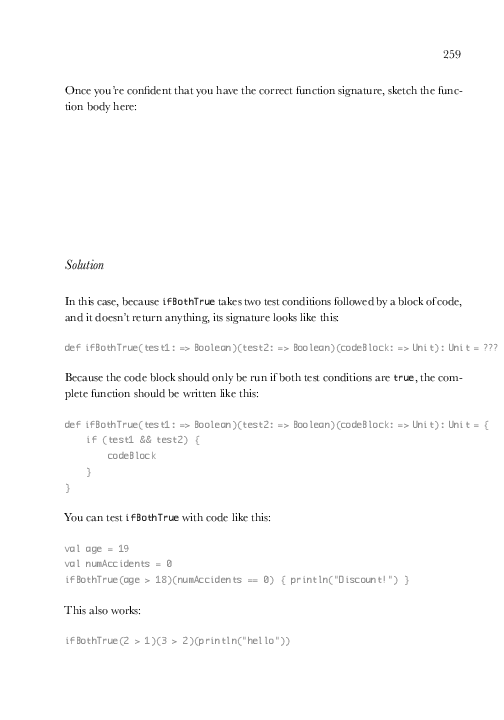
\includegraphics[height=2.51cm]{random-pages/random-pages-from-fpsimplified-pdf-00}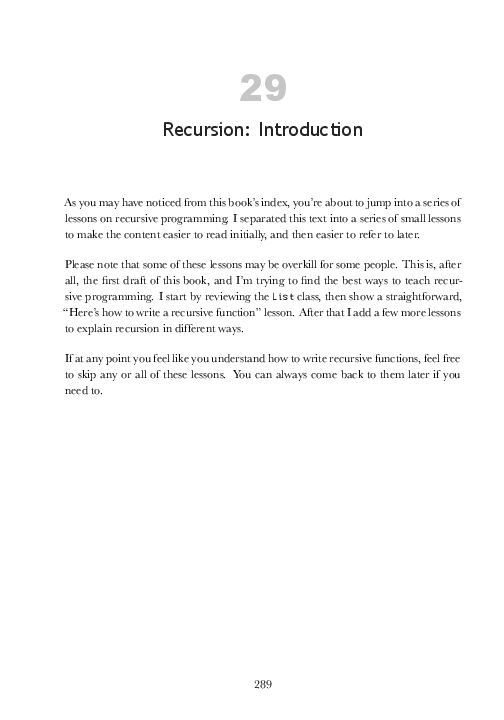
\includegraphics[height=2.51cm]{random-pages/random-pages-from-fpsimplified-pdf-01}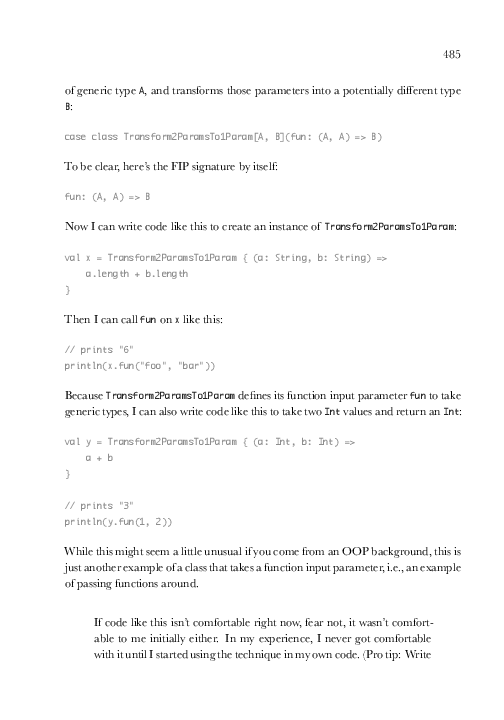
\includegraphics[height=2.51cm]{random-pages/random-pages-from-fpsimplified-pdf-02}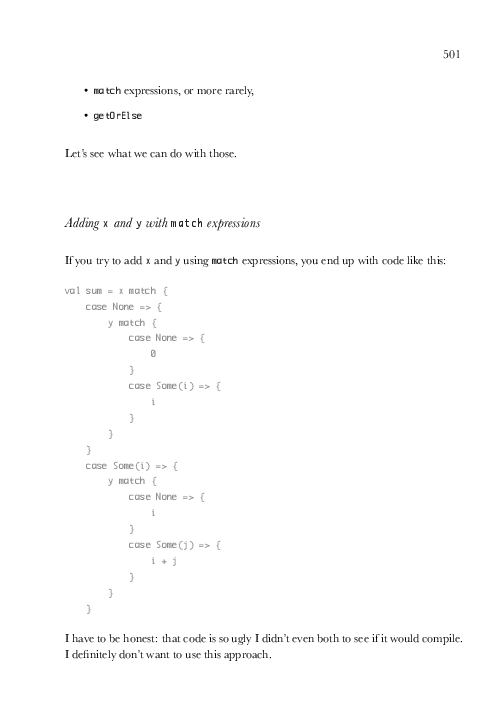
\includegraphics[height=2.51cm]{random-pages/random-pages-from-fpsimplified-pdf-03}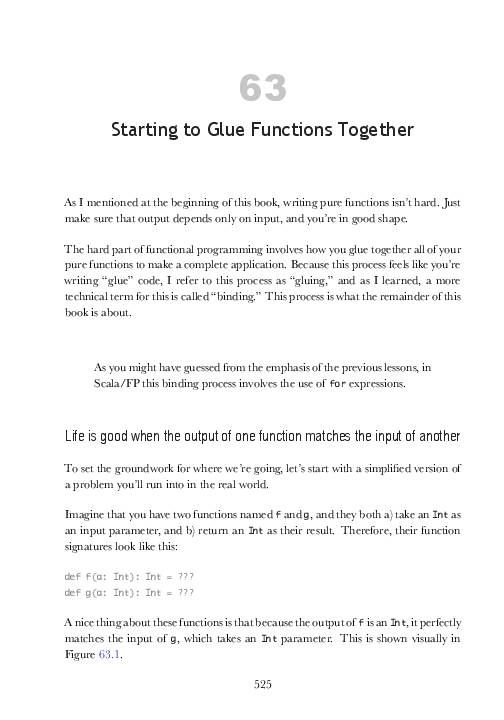
\includegraphics[height=2.51cm]{random-pages/random-pages-from-fpsimplified-pdf-04}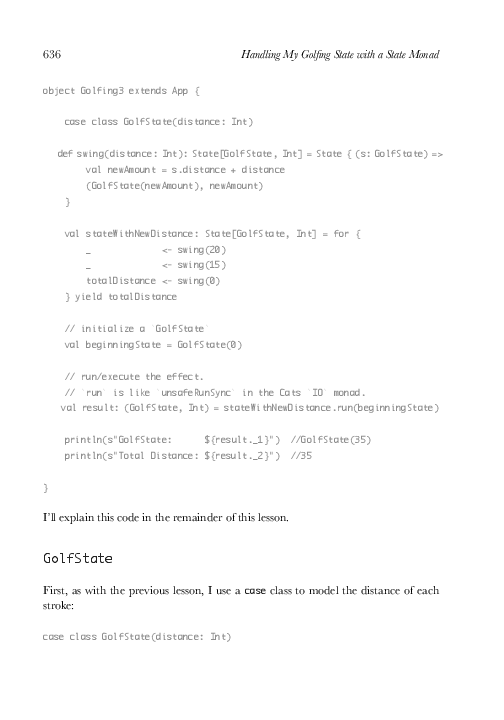
\includegraphics[height=2.51cm]{random-pages/random-pages-from-fpsimplified-pdf-05}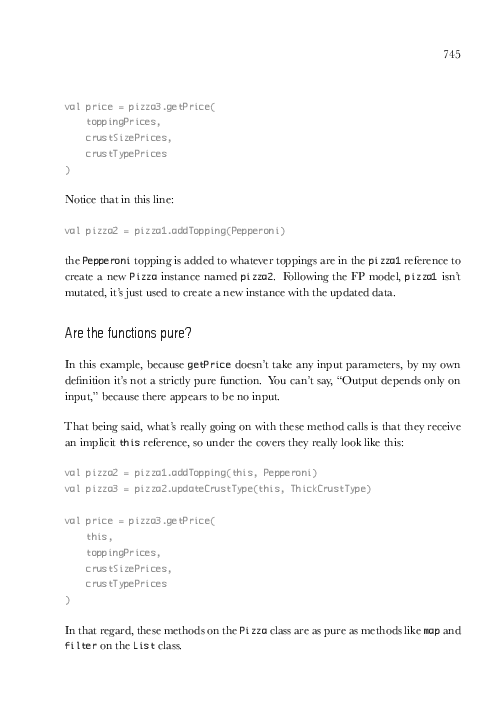
\includegraphics[height=2.51cm]{random-pages/random-pages-from-fpsimplified-pdf-06}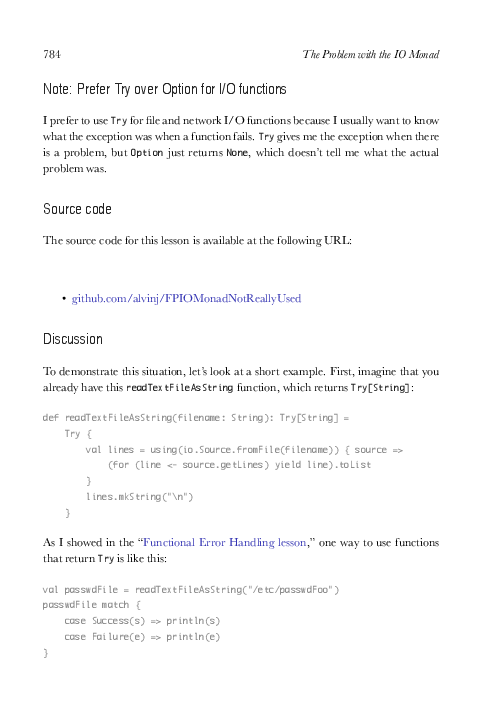
\includegraphics[height=2.51cm]{random-pages/random-pages-from-fpsimplified-pdf-07}
\par\end{centering}
\begin{centering}
\vspace{-0.3\baselineskip}
\par\end{centering}
\begin{centering}
\emph{Functional programming simplified}, by A.~Alexander
\par\end{centering}
\begin{centering}
\vspace{1\baselineskip}
\par\end{centering}
\begin{centering}
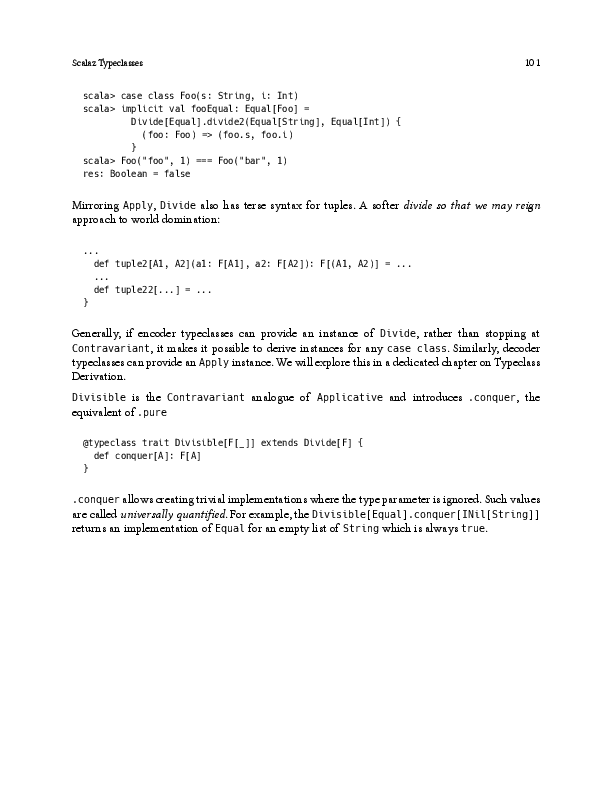
\includegraphics[height=2.51cm]{random-pages/random-pages-from-fpmortals-pdf-00}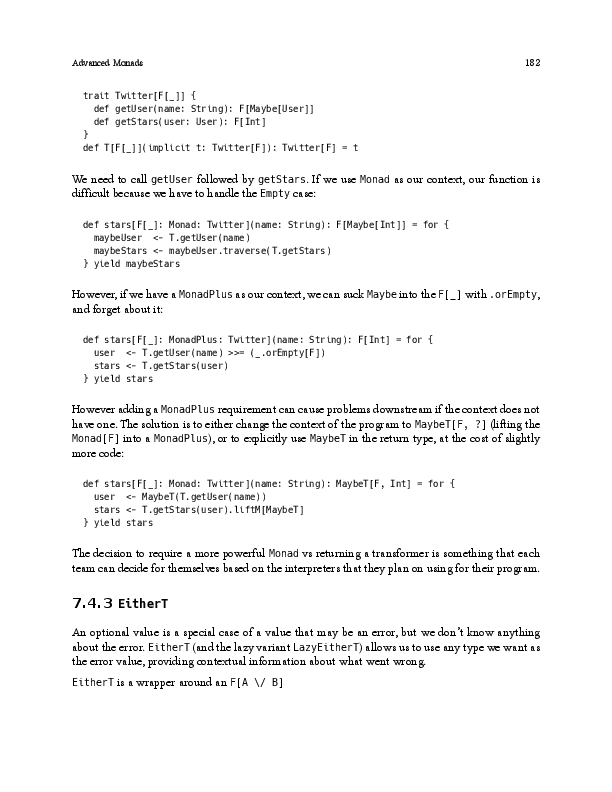
\includegraphics[height=2.51cm]{random-pages/random-pages-from-fpmortals-pdf-01}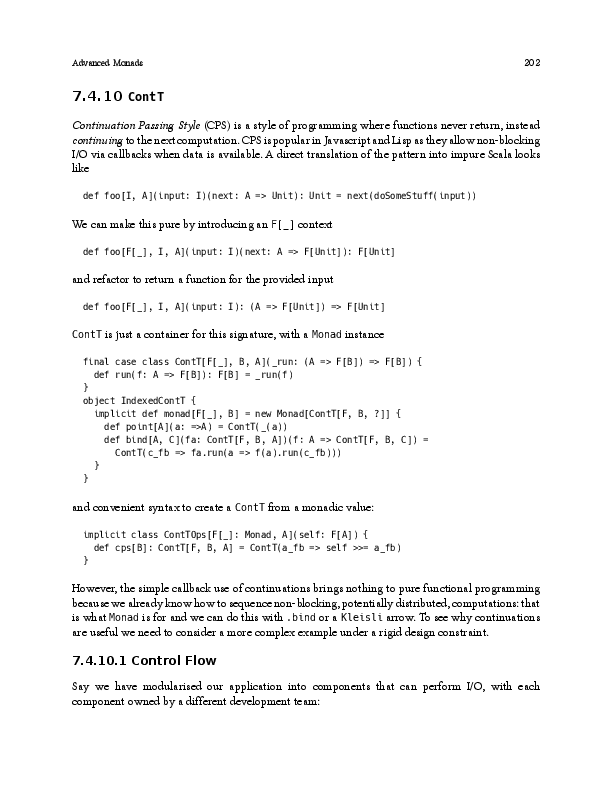
\includegraphics[height=2.51cm]{random-pages/random-pages-from-fpmortals-pdf-02}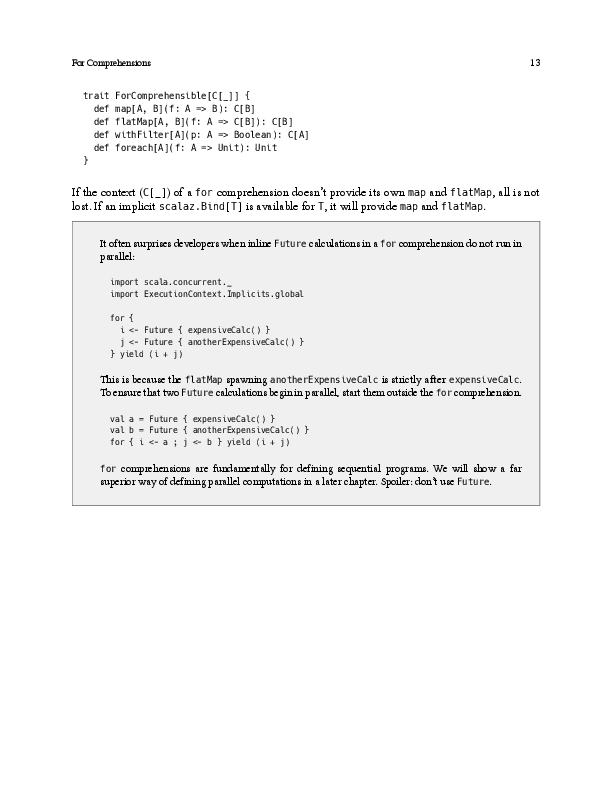
\includegraphics[height=2.51cm]{random-pages/random-pages-from-fpmortals-pdf-03}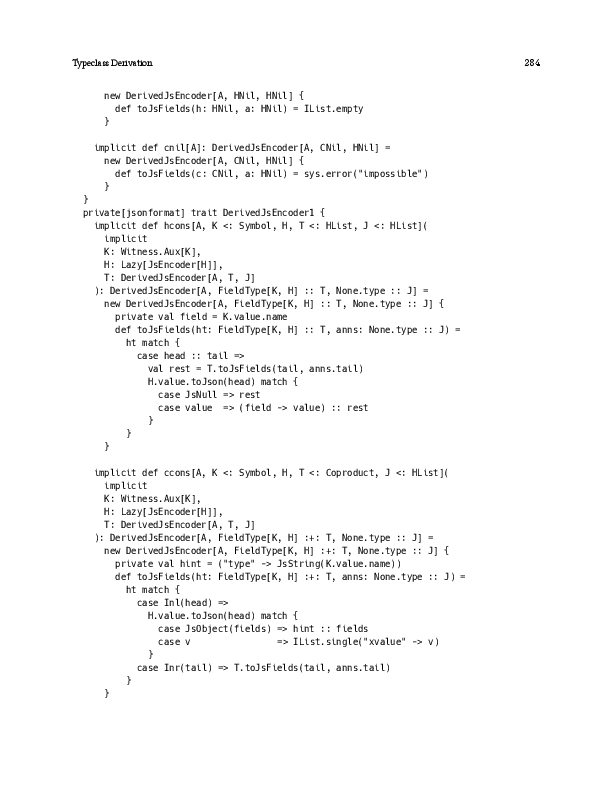
\includegraphics[height=2.51cm]{random-pages/random-pages-from-fpmortals-pdf-04}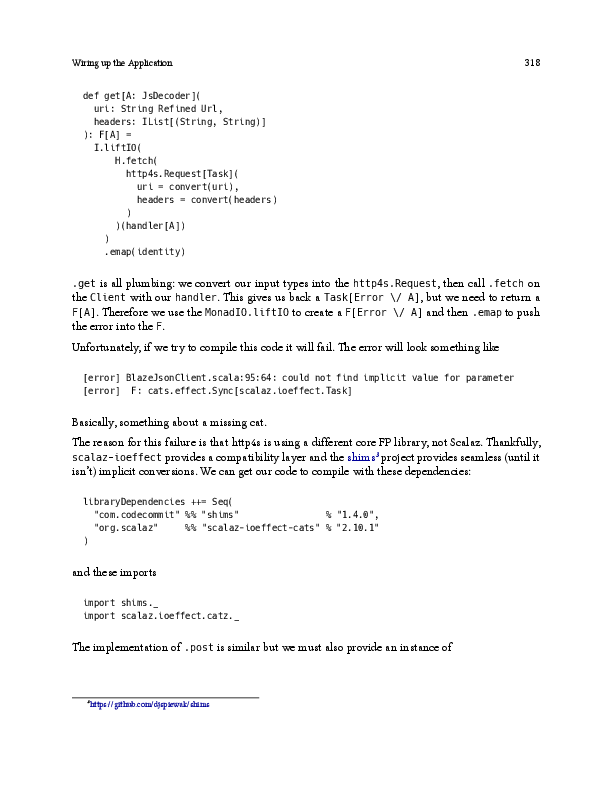
\includegraphics[height=2.51cm]{random-pages/random-pages-from-fpmortals-pdf-06}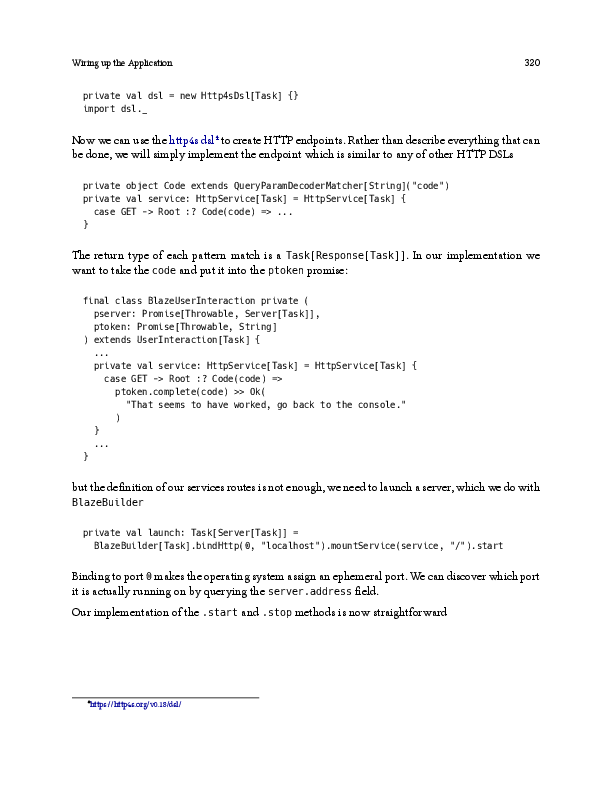
\includegraphics[height=2.51cm]{random-pages/random-pages-from-fpmortals-pdf-07}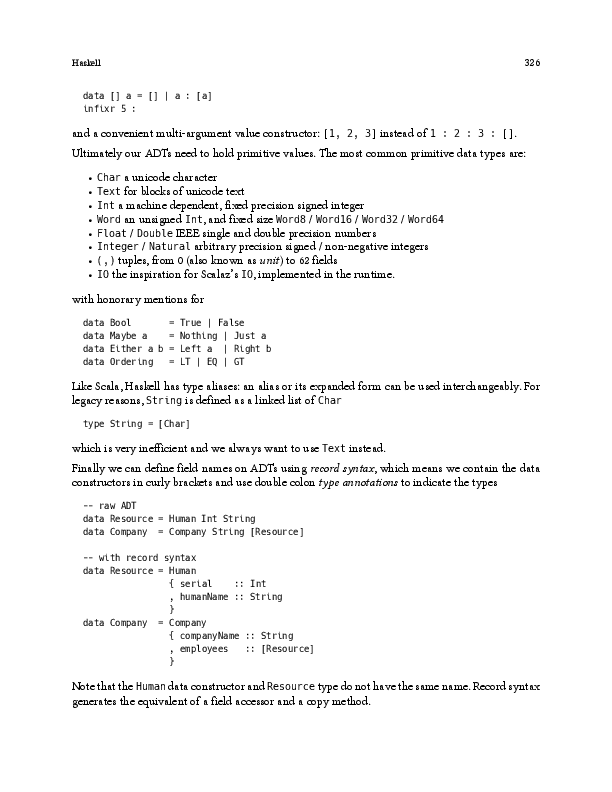
\includegraphics[height=2.51cm]{random-pages/random-pages-from-fpmortals-pdf-08}
\par\end{centering}
\begin{centering}
\emph{\vspace{-1.6\baselineskip}
}
\par\end{centering}
\begin{centering}
\emph{Functional programming for mortals}, by S.~Halliday
\par\end{centering}
\begin{centering}
\vspace{1\baselineskip}
\par\end{centering}
\begin{centering}
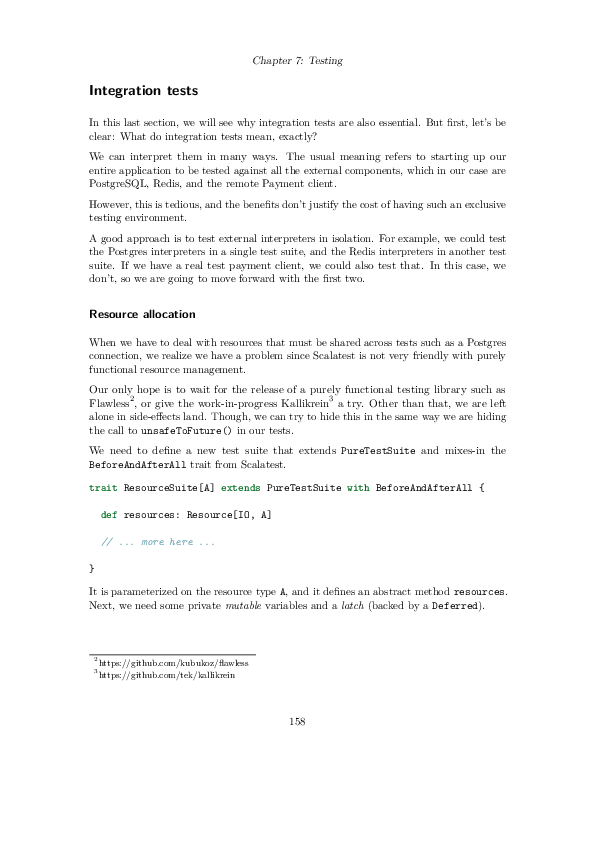
\includegraphics[height=2.51cm]{random-pages/random-pages-from-volpe-pdf-01}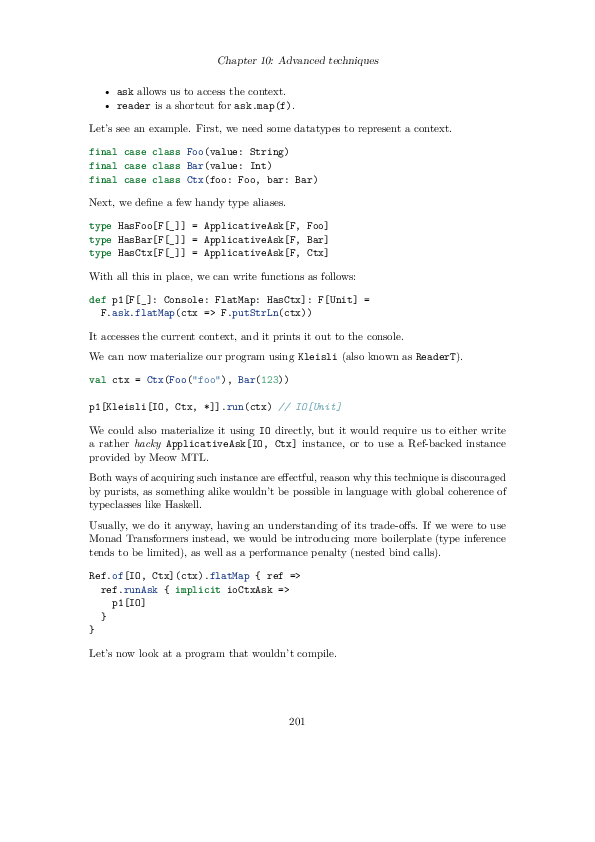
\includegraphics[height=2.51cm]{random-pages/random-pages-from-volpe-pdf-03}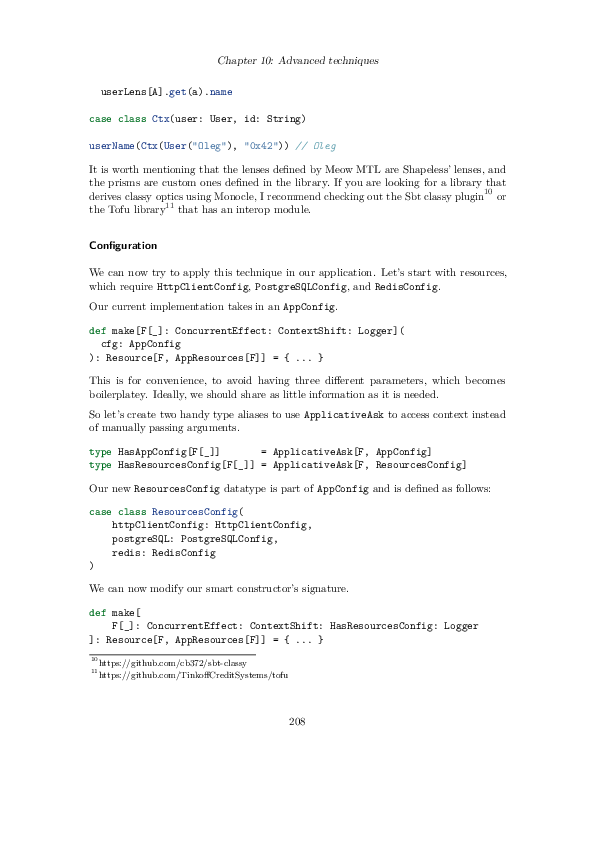
\includegraphics[height=2.51cm]{random-pages/random-pages-from-volpe-pdf-04}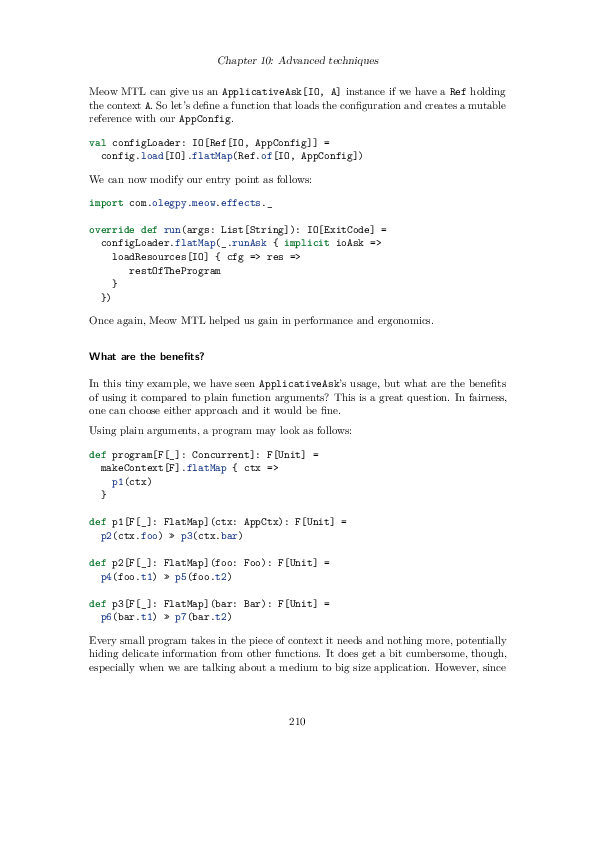
\includegraphics[height=2.51cm]{random-pages/random-pages-from-volpe-pdf-05}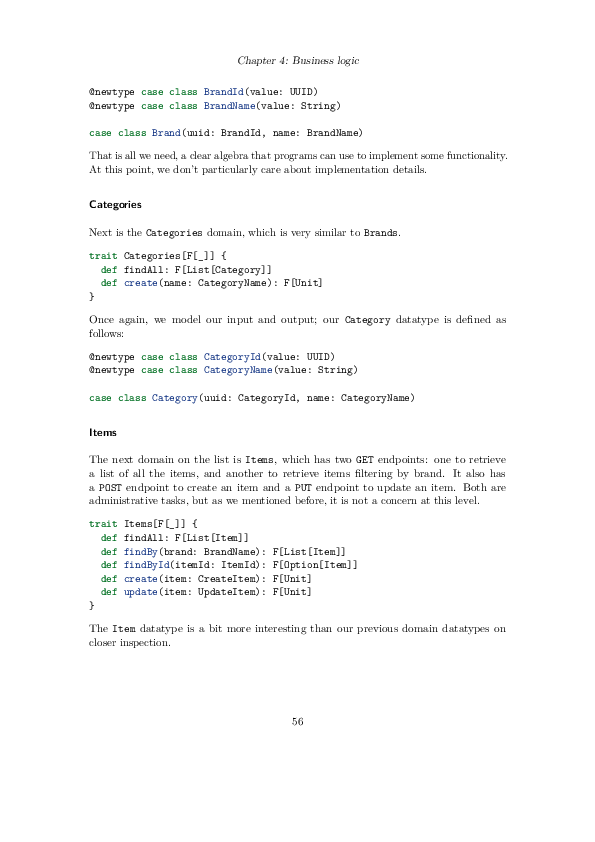
\includegraphics[height=2.51cm]{random-pages/random-pages-from-volpe-pdf-06}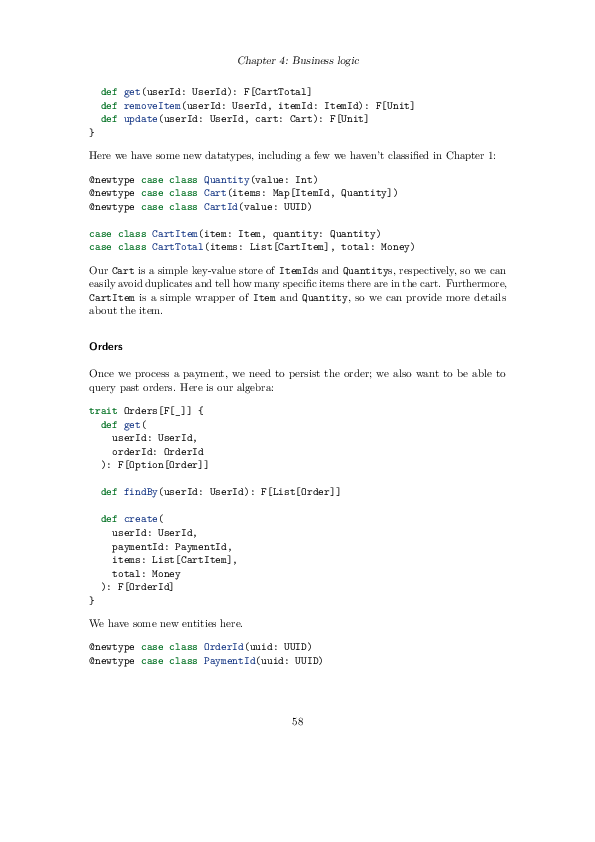
\includegraphics[height=2.51cm]{random-pages/random-pages-from-volpe-pdf-07}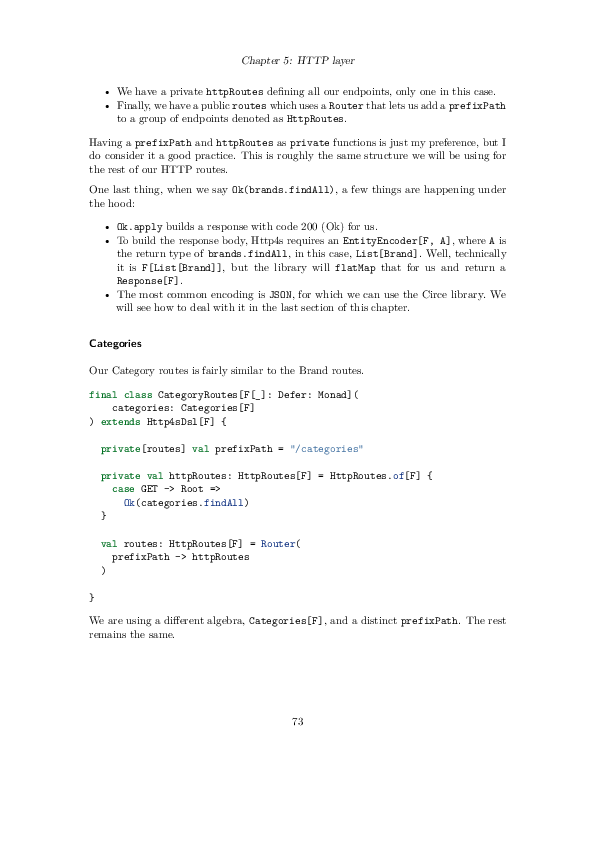
\includegraphics[height=2.51cm]{random-pages/random-pages-from-volpe-pdf-08}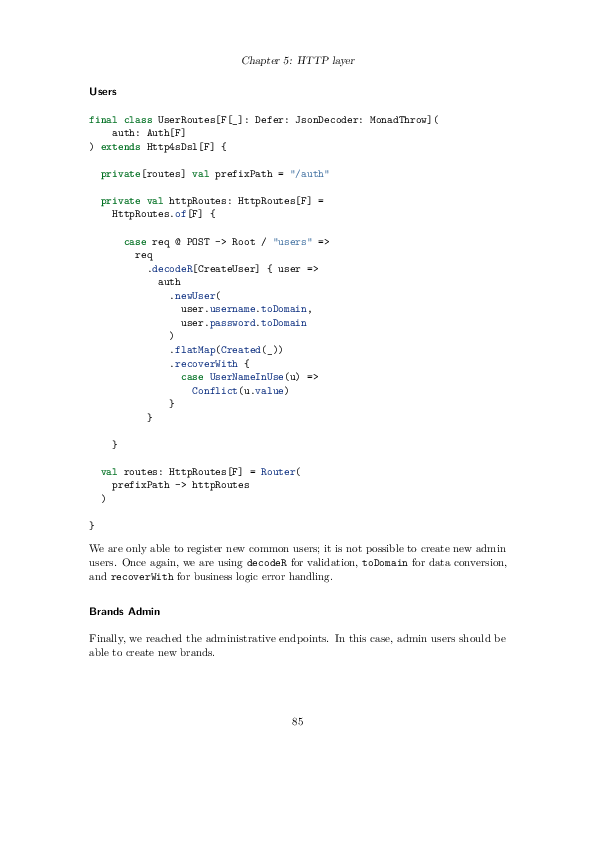
\includegraphics[height=2.51cm]{random-pages/random-pages-from-volpe-pdf-09}
\par\end{centering}
\begin{centering}
\emph{\vspace{-1.9\baselineskip}
}
\par\end{centering}
\begin{centering}
\emph{Practical functional programming in Scala}, by G.~Volpe (\texttt{\small{}\href{https://leanpub.com/pfp-scala}{https://leanpub.com/pfp-scala}})
\par\end{centering}
\begin{centering}
\vspace{1\baselineskip}
\par\end{centering}
\begin{centering}
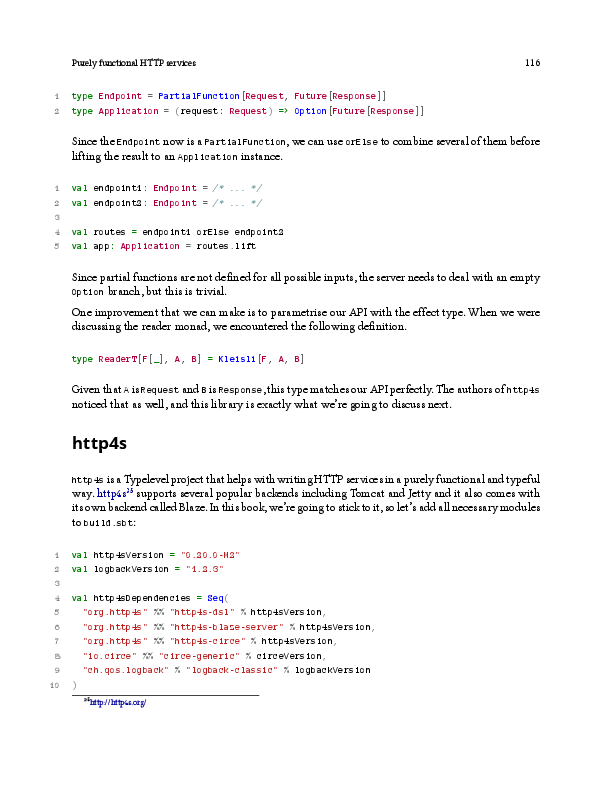
\includegraphics[height=2.51cm]{random-pages/random-pages-from-kalinin-pdf-01}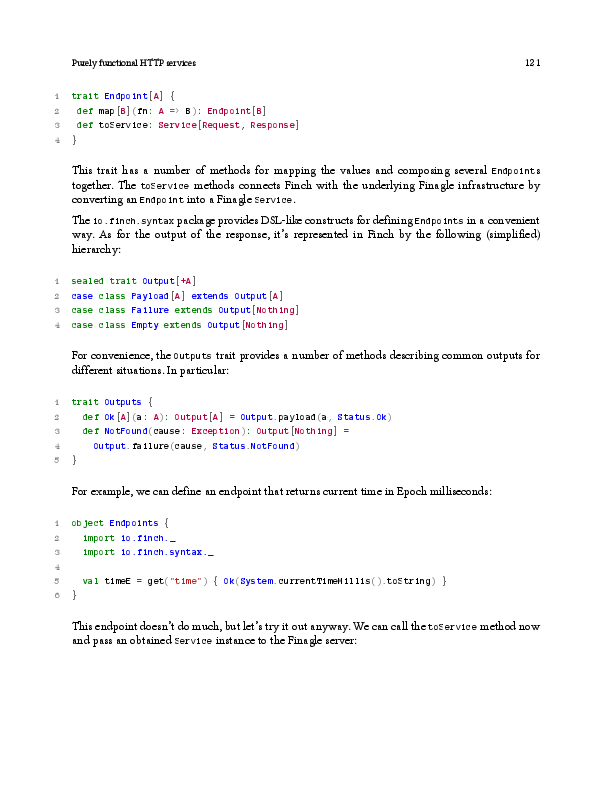
\includegraphics[height=2.51cm]{random-pages/random-pages-from-kalinin-pdf-02}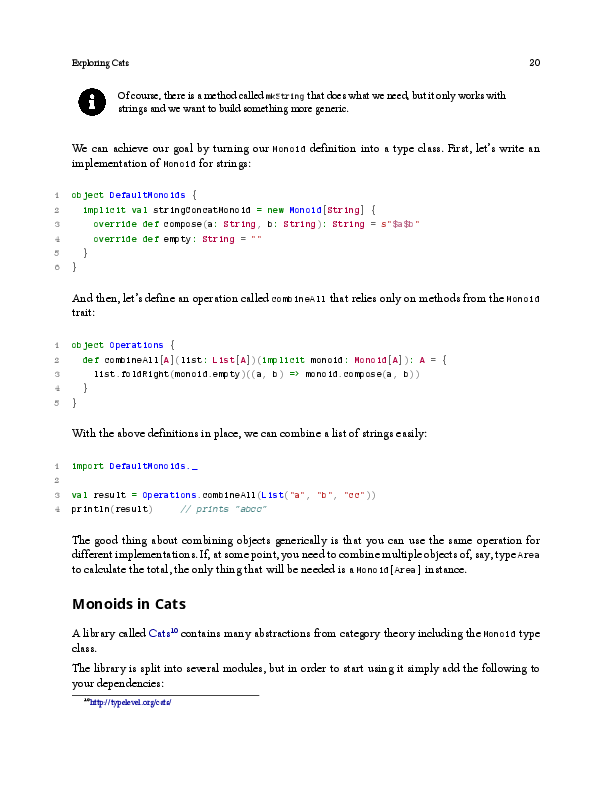
\includegraphics[height=2.51cm]{random-pages/random-pages-from-kalinin-pdf-03}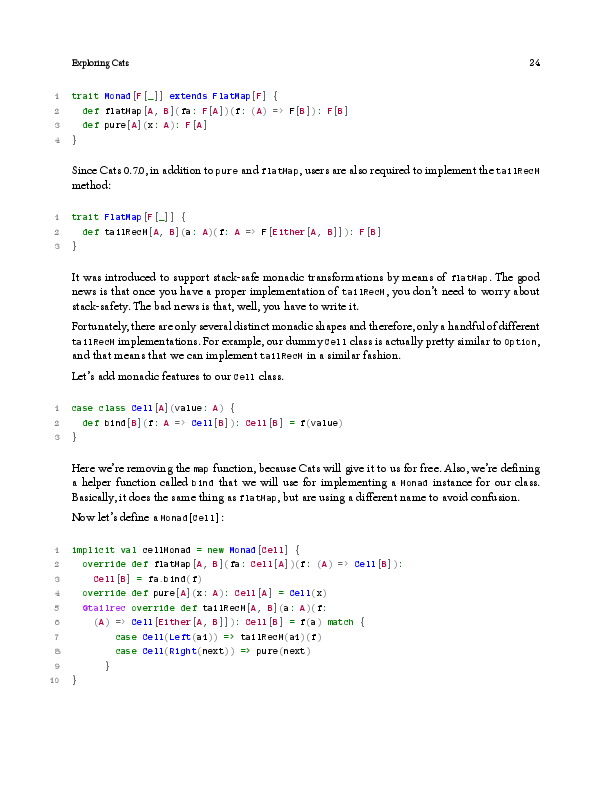
\includegraphics[height=2.51cm]{random-pages/random-pages-from-kalinin-pdf-04}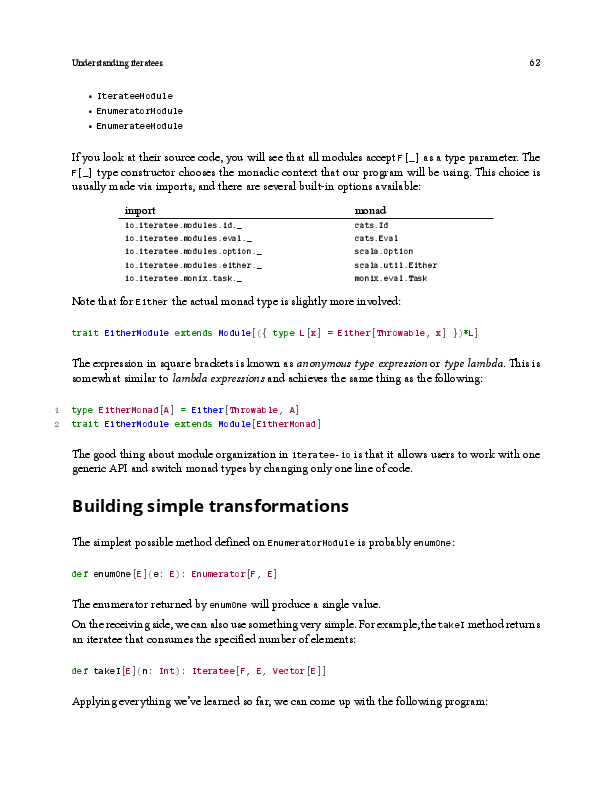
\includegraphics[height=2.51cm]{random-pages/random-pages-from-kalinin-pdf-06}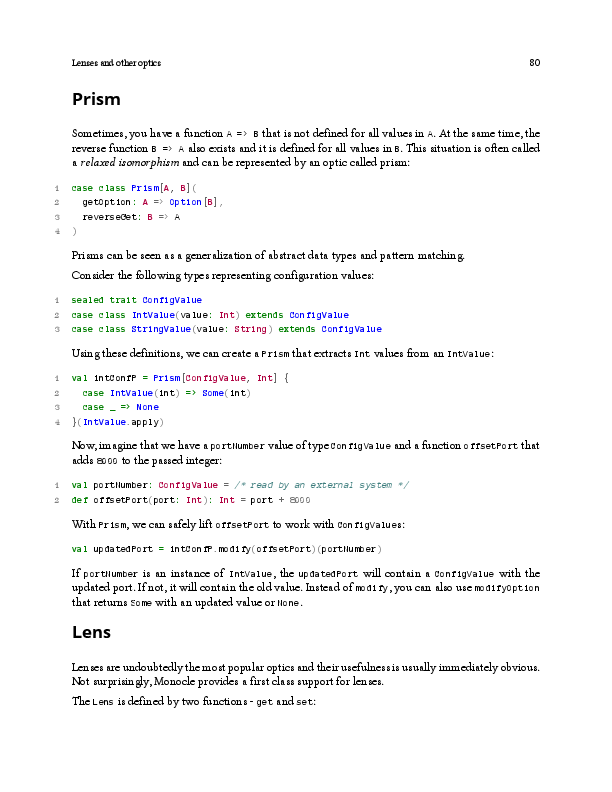
\includegraphics[height=2.51cm]{random-pages/random-pages-from-kalinin-pdf-07}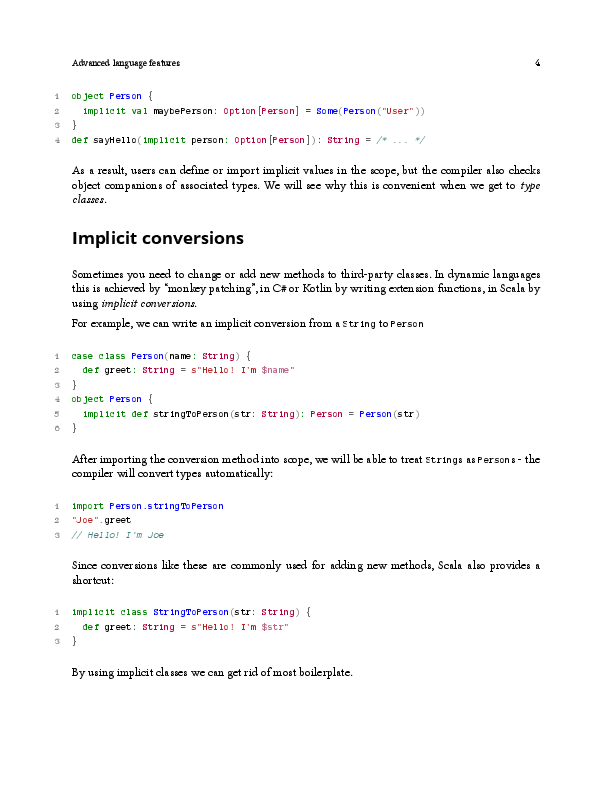
\includegraphics[height=2.51cm]{random-pages/random-pages-from-kalinin-pdf-08}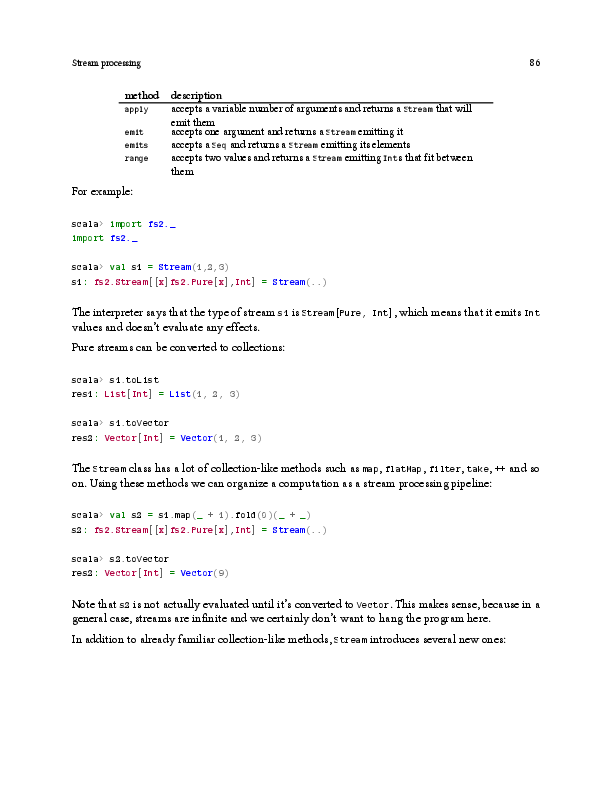
\includegraphics[height=2.51cm]{random-pages/random-pages-from-kalinin-pdf-09}
\par\end{centering}
\vspace{-0.6\baselineskip}

\begin{centering}
\emph{Mastering advanced Scala}, by D.~Kalinin (\texttt{\small{}\href{https://leanpub.com/mastering-advanced-scala}{https://leanpub.com/mastering-advanced-scala}})
\par\end{centering}
\caption{Randomly chosen pages from books on Scala programming.\label{fig:Randomly-chosen-pages-1}}
\end{figure}

\begin{figure}
\begin{centering}
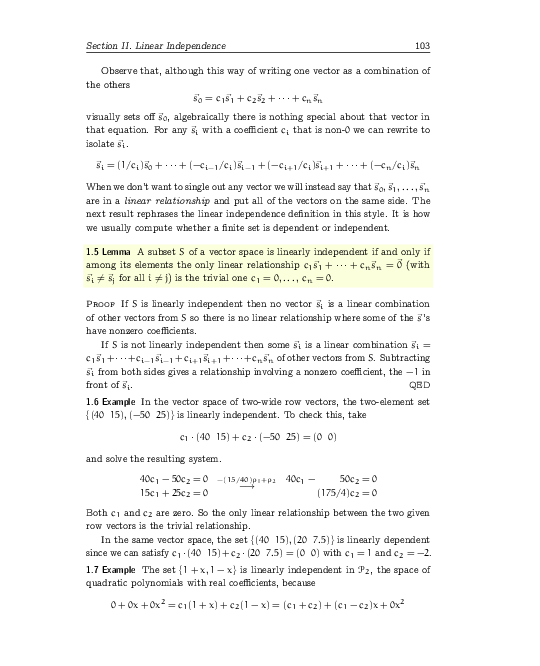
\includegraphics[height=2.51cm]{random-pages/random-pages-from-hefferon-pdf-00}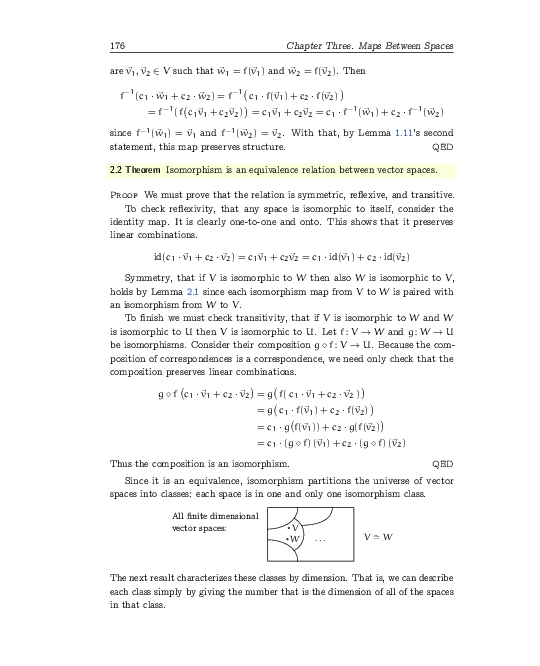
\includegraphics[height=2.51cm]{random-pages/random-pages-from-hefferon-pdf-01}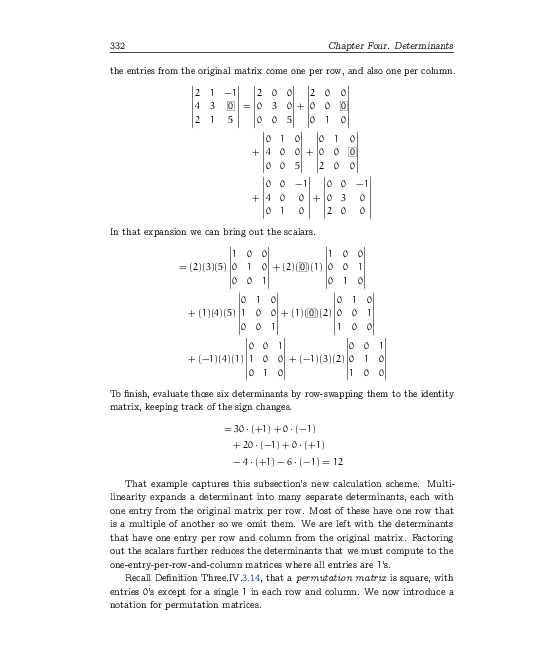
\includegraphics[height=2.51cm]{random-pages/random-pages-from-hefferon-pdf-03}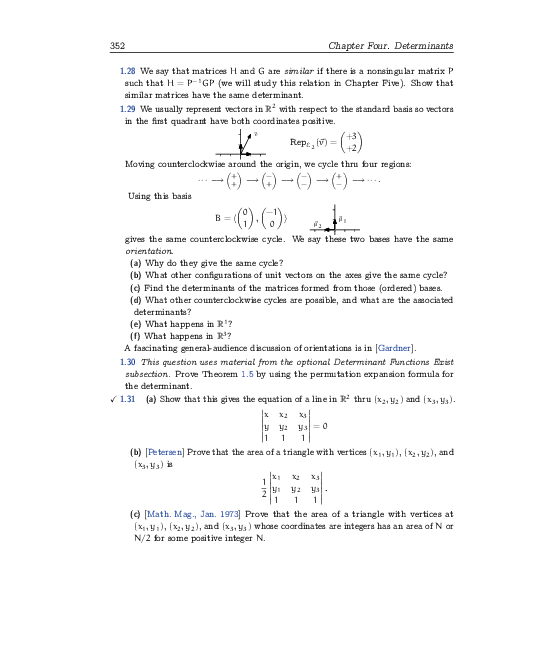
\includegraphics[height=2.51cm]{random-pages/random-pages-from-hefferon-pdf-04}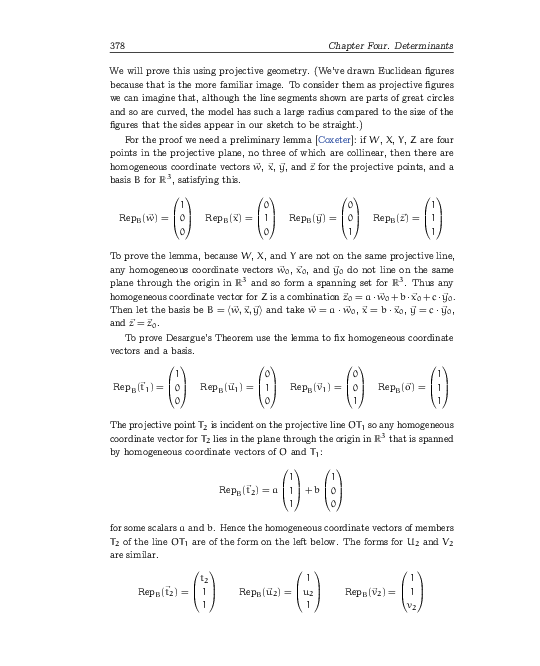
\includegraphics[height=2.51cm]{random-pages/random-pages-from-hefferon-pdf-05}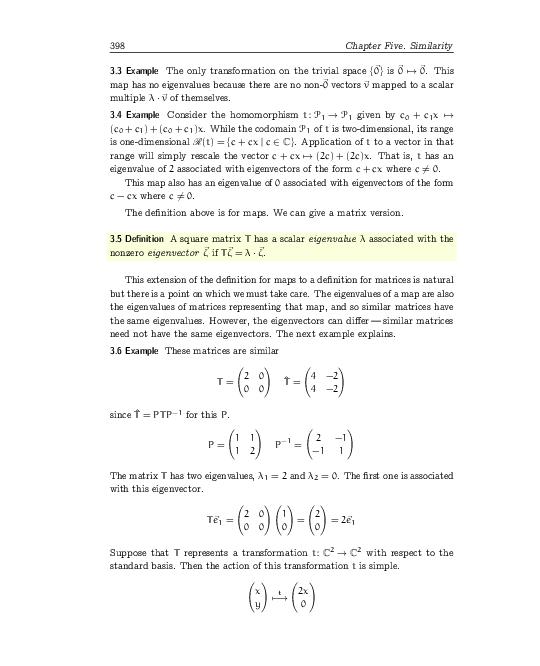
\includegraphics[height=2.51cm]{random-pages/random-pages-from-hefferon-pdf-06}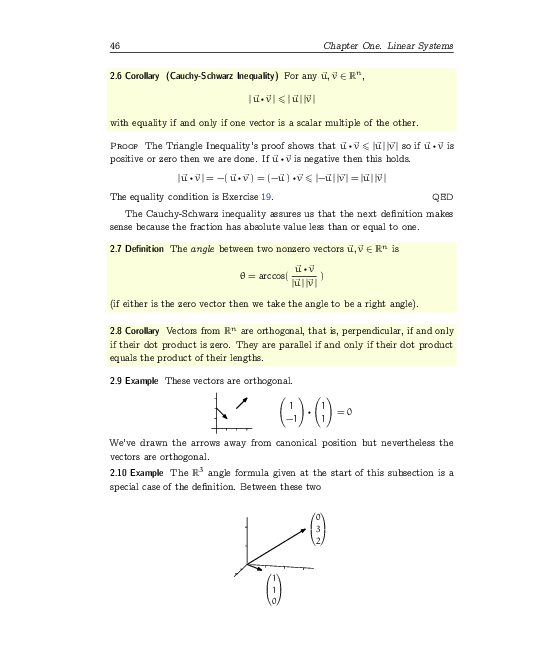
\includegraphics[height=2.51cm]{random-pages/random-pages-from-hefferon-pdf-07}
\par\end{centering}
\vspace{-0.4\baselineskip}

\begin{centering}
\emph{Linear algebra}, by J.~Hefferon (\texttt{\small{}\href{http://joshua.smcvt.edu/linearalgebra/}{http://joshua.smcvt.edu/linearalgebra/}})
\par\end{centering}
\begin{centering}
\vspace{0.6\baselineskip}
\par\end{centering}
\begin{centering}
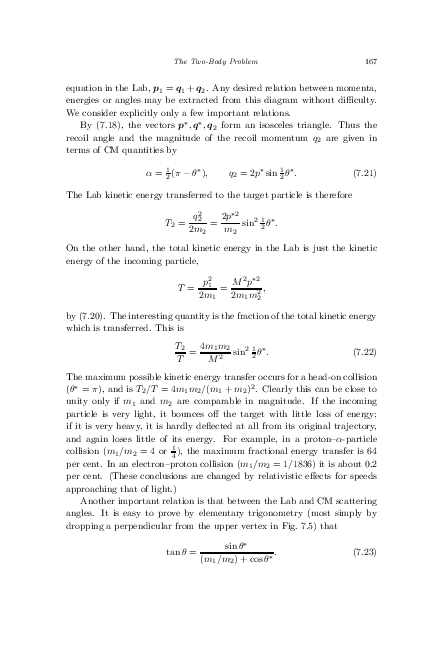
\includegraphics[height=2.51cm]{random-pages/random-pages-from-kibble-pdf-00}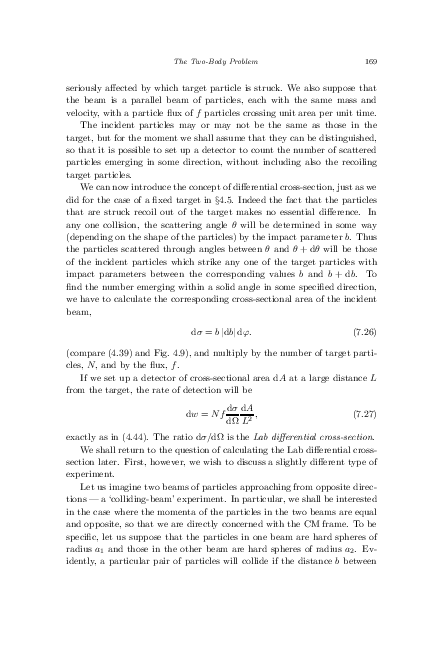
\includegraphics[height=2.51cm]{random-pages/random-pages-from-kibble-pdf-01}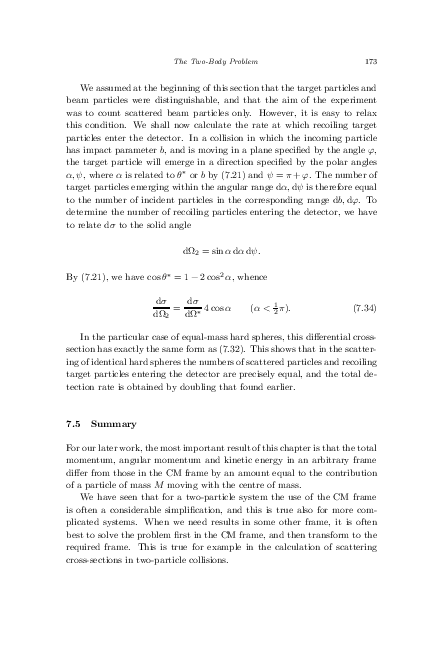
\includegraphics[height=2.51cm]{random-pages/random-pages-from-kibble-pdf-02}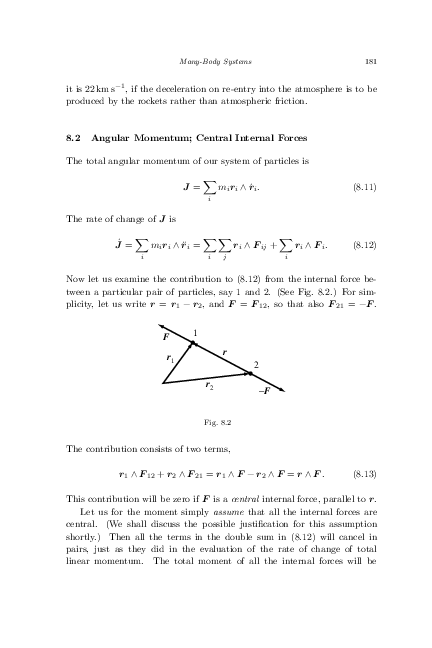
\includegraphics[height=2.51cm]{random-pages/random-pages-from-kibble-pdf-03}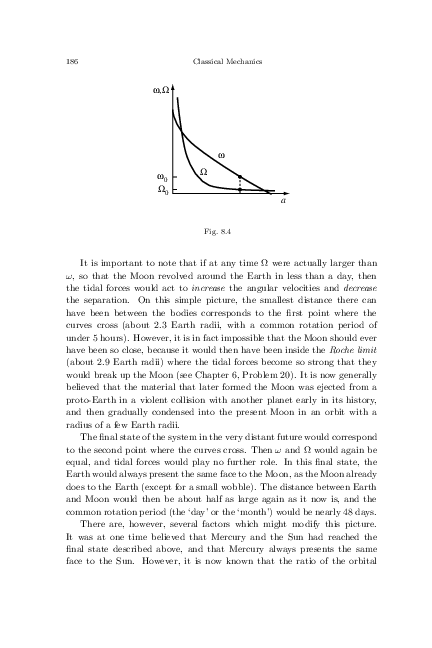
\includegraphics[height=2.51cm]{random-pages/random-pages-from-kibble-pdf-04}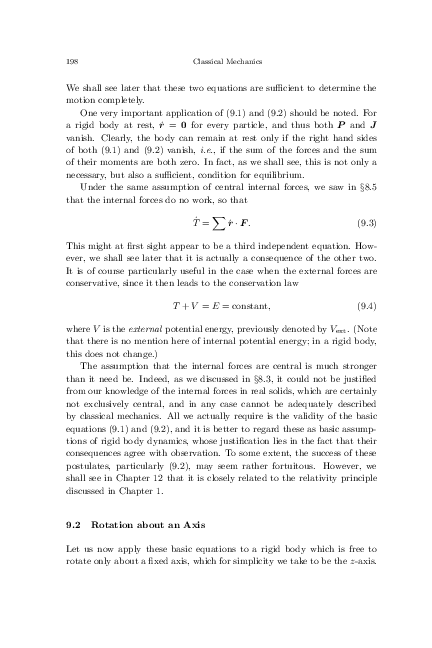
\includegraphics[height=2.51cm]{random-pages/random-pages-from-kibble-pdf-05}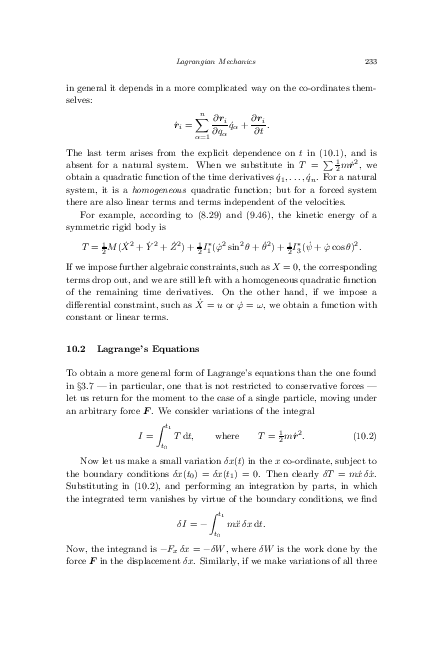
\includegraphics[height=2.51cm]{random-pages/random-pages-from-kibble-pdf-06}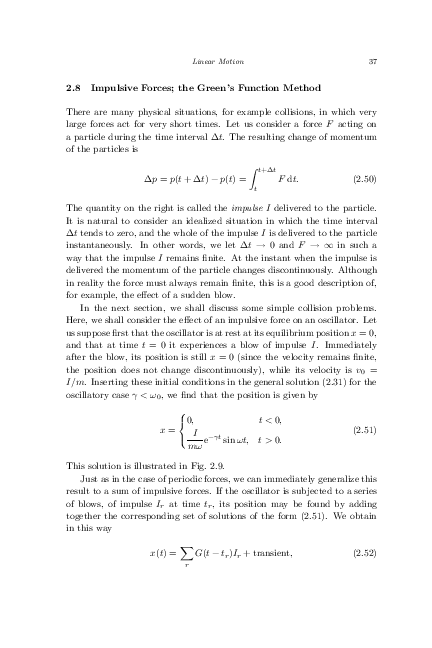
\includegraphics[height=2.51cm]{random-pages/random-pages-from-kibble-pdf-09}
\par\end{centering}
\vspace{-0.6\baselineskip}

\begin{centering}
\emph{Classical mechanics}, by T.~W.~B.~Kibble and F.~H.~Berkshire
(\texttt{\small{}\href{https://archive.org/details/116772449ClassicalMechanics}{https://archive.org/details/116772449ClassicalMechanics}})
\par\end{centering}
\vspace{0.6\baselineskip}

\caption{Randomly chosen pages from books on mathematics and physics.\label{fig:Randomly-chosen-pages-2}}
\end{figure}

\begin{figure}
\begin{centering}
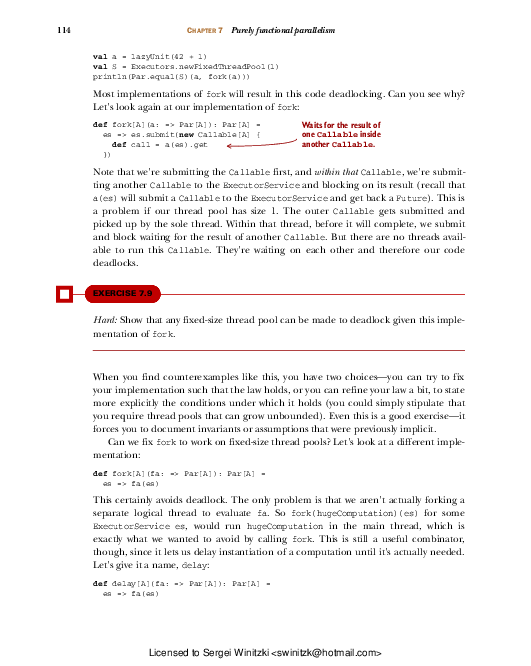
\includegraphics[height=2.51cm]{random-pages/random-pages-from-fpis-pdf-00}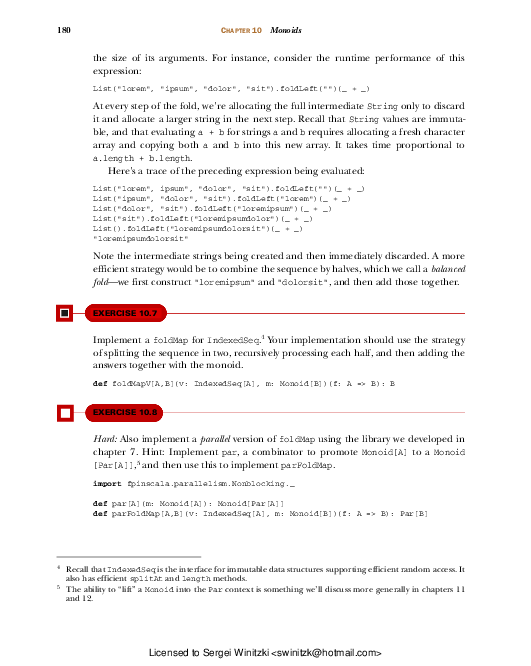
\includegraphics[height=2.51cm]{random-pages/random-pages-from-fpis-pdf-02}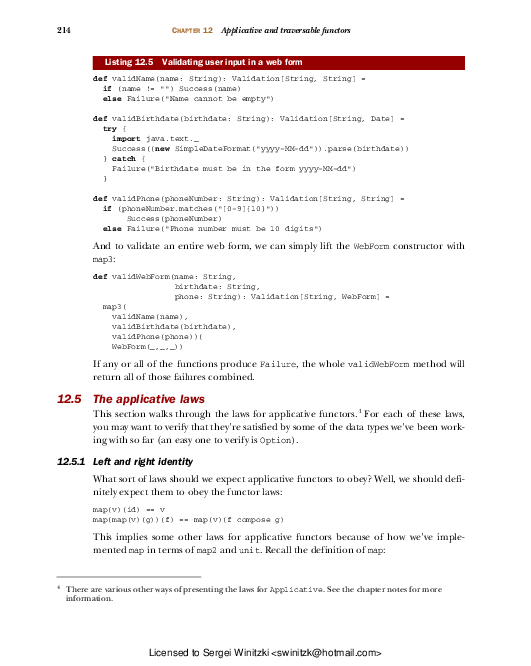
\includegraphics[height=2.51cm]{random-pages/random-pages-from-fpis-pdf-04}\includegraphics[height=2.51cm]{random-pages/random-pages-from-fpis-pdf-05}\includegraphics[height=2.51cm]{random-pages/random-pages-from-fpis-pdf-06}\includegraphics[height=2.51cm]{random-pages/random-pages-from-fpis-pdf-07}\includegraphics[height=2.51cm]{random-pages/random-pages-from-fpis-pdf-08}
\par\end{centering}
\vspace{-0\baselineskip}

\begin{centering}
\emph{Functional programming in Scala}, by P.~Chiusano and R.~Bjarnason
\par\end{centering}
\begin{centering}
\vspace{1\baselineskip}
\par\end{centering}
\begin{centering}
\includegraphics[height=2.51cm]{random-pages/random-pages-from-pdbc-pdf-00}\includegraphics[height=2.51cm]{random-pages/random-pages-from-pdbc-pdf-01}\includegraphics[height=2.51cm]{random-pages/random-pages-from-pdbc-pdf-02}\includegraphics[height=2.51cm]{random-pages/random-pages-from-pdbc-pdf-03}\includegraphics[height=2.51cm]{random-pages/random-pages-from-pdbc-pdf-04}\includegraphics[height=2.51cm]{random-pages/random-pages-from-pdbc-pdf-05}\includegraphics[height=2.51cm]{random-pages/random-pages-from-pdbc-pdf-06}\includegraphics[height=2.51cm]{random-pages/random-pages-from-pdbc-pdf-07}
\par\end{centering}
\vspace{-0.7\baselineskip}

\begin{centering}
\emph{Program design by calculation}, by J.~N.~Oliveira
\par\end{centering}
\begin{centering}
\vspace{1\baselineskip}
\par\end{centering}
\begin{centering}
\includegraphics[height=2.51cm]{random-pages/random-pages-from-sofp-pdf-00}\includegraphics[height=2.51cm]{random-pages/random-pages-from-sofp-pdf-01}\includegraphics[height=2.51cm]{random-pages/random-pages-from-sofp-pdf-02}\includegraphics[height=2.51cm]{random-pages/random-pages-from-sofp-pdf-05}\includegraphics[height=2.51cm]{random-pages/random-pages-from-sofp-pdf-06}\includegraphics[height=2.51cm]{random-pages/random-pages-from-sofp-pdf-07}\includegraphics[height=2.51cm]{random-pages/random-pages-from-sofp-pdf-08}
\par\end{centering}
\vspace{-0.3\baselineskip}

\begin{centering}
\emph{The science of functional programming} (this book)
\par\end{centering}
\vspace{1\baselineskip}

\caption{Randomly chosen pages from books on applied functional type theory.\label{fig:Randomly-chosen-pages}}
\end{figure}


\addchap{Essay: Why category theory is useful in functional programming}

\index{category theory!in functional programming}This essay is for
readers who are already somewhat familiar with category theory.

\addsec{A \textquotedblleft types/functions\textquotedblright{} category for
a programming language}

We consider programming languages that support various data types,
such as integers (\lstinline!Int!), floating-point numbers (\lstinline!Float!),
strings (\lstinline!String!), arrays of strings (\lstinline!Array[String]!),
and so on. Such languages allow programmers to define functions with
specified types of arguments and return values. The compiler will
then verify that all functions are always applied to arguments of
correct types, and also that all return values have the expected types. 

To each programming language of that kind, there corresponds\footnote{Academically minded computer scientists say that this definition of
a \textsf{``}types/functions\textsf{''} category is insufficiently rigorous. See the
discussion in \texttt{\href{https://math.andrej.com/2016/08/06/hask-is-not-a-category/}{https://math.andrej.com/2016/08/06/hask-is-not-a-category/}}} a \textsf{``}types/functions\textsf{''} category:
\begin{itemize}
\item The objects of the category are all the data types supported by the
language (including user-defined data types). As an example, for Scala
there will be an object \lstinline!Int!, an object \lstinline!Float!,
an object \lstinline!String!, an object \lstinline!Array[String]!,
and so on.
\item The morphisms between objects \lstinline!A! and \lstinline!B! are
all functions implementable in the language (with finitely long program
code) that take a single argument of type \lstinline!A! and return
a value of type \lstinline!B!.
\item We assume that the computer has countably infinite memory, so objects
can be viewed as (at most) countably infinite sets. Morphisms will
also form at most countably infinite sets.
\end{itemize}
The category defined in this way will typically have a large number
of morphisms between most objects. For example, morphisms between
objects \lstinline!Boolean! and \lstinline!Int! are functions that
take a single argument of type \lstinline!Boolean! and return a value
of type \lstinline!Int!. There are as many such functions as pairs
of integers. Scala code for one of those morphisms looks like this:
\begin{lstlisting}
def morphismBooleanToInt: Boolean => Int = { b => if (b) 123 else 456 }
\end{lstlisting}

Why do the category laws hold? The composition of morphisms corresponds
to composition of functions, which we can implement by writing code
that applies the first function and then applies the second function.
In Scala:
\begin{lstlisting}
def composeMorphisms[A, B, C](f: A => B, g: B => C): A => C   =   { a => g(f(a)) }
\end{lstlisting}
Equivalent functionality can be implemented in most programming languages.

The category\textsf{'}s identity law says that there must be a morphism between
objects \lstinline!A! and \lstinline!A!. This can be implemented
in most programming languages as a function that returns its argument
unchanged:
\begin{lstlisting}
def identity[A]: A => A = { x => x }
\end{lstlisting}
One can check that morphism composition is associative and agrees
with the identity morphism.

For a given programming language, we have thus defined the \textsf{``}types/functions
category\textsf{''}, which can be seen as a subcategory of the category of
sets. Most of the time, we will be working with that category, or
with the category of its endofunctors, or with a sub-category of these
categories.

Different programming languages will give rise to different \textsf{``}types/functions\textsf{''}
categories, but all those categories have many common features that
are especially important in languages designed for functional programming
(the \textsf{``}FP languages\textsf{''}, such as OCaml, Haskell, Scala and others).

\addsec{The use of endofunctors}

An endofunctor in the \textsf{``}types/functions\textsf{''} category is a mapping
of types together with a mapping of functions. A good example is the
\lstinline!Array! data type. In some programming languages, the type
of an array\textsf{'}s elements can be specified and enforced throughout the
code. For example, in Scala one can use the type \lstinline!Array[Int]!
for an array of integers, \lstinline!Array[String]! for an array
of strings, \lstinline!Array[Array[Int]]! for an array containing
nested arrays of integers, etc. So, \lstinline!Array! can be seen
as a mapping from types to types: it maps the type \lstinline!Int!
to the type \lstinline!Array[Int]!, the type \lstinline!String!
to the type \lstinline!Array[String]!, etc. For any type \lstinline!X!,
we have the type \lstinline!Array[X]!. This is the object-to-object
map of an endofunctor.

An endofunctor also needs a map from morphisms to morphisms. Given
a function \lstinline!f: X => Y!, we need to implement a function
of type \lstinline!Array[X] => Array[Y]!. This can be done by writing
a loop over the array and applying the function \lstinline!f! to
each element (of type \lstinline!X!). The resulting values (of type
\lstinline!Y!) are then collected in a new array, of type \lstinline!Array[Y]!.

This code can be written in many programming languages in a generic
manner, using type parameters such as \lstinline!X! and \lstinline!Y!.
The same code will then work for arrays and functions of any given
type. In Scala, the code could be written as the following function
(usually called \lstinline!fmap! in FP libraries):
\begin{lstlisting}
def fmap[X, Y: ClassTag](f: X => Y): Array[X] => Array[Y] = { arrayX: Array[X] =>
  val arrayY = new Array[Y](arrayX.size)
  for { i <- arrayX.indices } arrayY(i) = f(arrayX(i))
  arrayY  // Return this array of type Array[Y].
}
\end{lstlisting}
One can then check that the code of \lstinline!fmap! satisfies the
identity and composition laws of endofunctors. This completes the
implementation of the \lstinline!Array! endofunctor.

Why does \lstinline!fmap! satisfy the laws of endofunctors? The categorical
properties of functions are preserved if we apply functions to each
element of an array and collect the results \emph{in the same order}.
An identity function applied to every element will not modify the
array. Function composition is preserved because a composition of
two functions will be applied separately to each array element.

The same construction can be applied to many data structures other
than arrays. It turns out that many programs can be reformulated using
the operation of applying a function to every value in a data structure
(i.e., the function \lstinline!fmap!). This reformulation leads to
code that avoids loops: the loops are replaced by \lstinline!fmap!
functions of some endofunctors, and all those \lstinline!fmap! functions
are implemented in a standard library. In practice, code written via
\lstinline!fmap! instead of loops is more concise and admits fewer
opportunities for errors. The programmer\textsf{'}s intuition about \textsf{``}applying
functions to every value held within a data structure\textsf{''} is then directly
represented by the formal laws of endofunctors. Once those laws are
verified, the programmer is assured that the code written via \lstinline!fmap!
will work according to the programmer\textsf{'}s intuitive expectations.

\addsec{The use of natural transformations}

What is a natural transformation between endofunctors in the \textsf{``}types/functions\textsf{''}
category? For two given endofunctors \lstinline!F! and \lstinline!G!,
a natural transformation \lstinline!t: F ~> G! is defined by its
components. The component at object \lstinline!X! is a function of
type \lstinline!F[X] => G[X]!; this must be defined for all \lstinline!X!.
Some programming languages support functions with type parameters.
In Scala, the syntax is
\begin{lstlisting}
def t[X]: F[X] => G[X] = ...
\end{lstlisting}
The code of such a function is written once and will work in the same
way for all types \lstinline!X!.

An example of natural transformation is a function that reverses the
order of elements in an array:
\begin{lstlisting}
def reverse[X]: Array[X] => Array[X] = ...
\end{lstlisting}
The algorithm is \textsf{``}fully parametric\textsf{''}: it is written in the same
way for all type parameters \lstinline!X!.

It turns out that, by the Reynolds-Wadler parametricity theorem, any
code written in a fully parametric manner will satisfy the law of
a natural transformation (the naturality law). The naturality law
states that applying the endofunctor \lstinline!F!\textsf{'}s morphism map
before a natural transformation \lstinline!t! must be equal to applying
the endofunctor \lstinline!G!\textsf{'}s map after \lstinline!t!. In Scala
syntax, the law is written as
\begin{lstlisting}
t(fmap_F(f)(x)) == fmap_G(f)(t(x))
\end{lstlisting}
This law can be verified directly for a given code of \lstinline!t!
and with known code for \lstinline!fmap_F! and \lstinline!fmap_G!.

Naturality laws are satisfied by transformations that rearrange data
items in a data structure in some way that does not depend on specific
values or types. In this way, the formal laws of natural transformations
directly represent programmers\textsf{'} intuitions about code that works \textsf{``}in
the same way for all type parameters\textsf{''}.

As we have just seen, the notions of endofunctors and natural transformations
are useful in programming languages that support types with type parameters
(such as \lstinline!Array[X]!) and functions with type parameters
(such as \lstinline!reverse[X]!). Programming languages that do not
support those features cannot benefit from the powerful reasoning
tools of category theory.

\addsec{Other properties of the \textquotedblleft types/functions\textquotedblright{}
category}

Morphisms in the \textsf{``}types/functions\textsf{''} category are always functions
of a single argument. However, programming languages usually support
functions with many arguments. There are two ways to imitate such
functions: tupling and currying.

Tupling means that we put all arguments into a compound structure
(a pair, a triple, etc.). The function is still viewed as having a
single argument, but the type of that argument is the type of a pair,
or a triple, or a longer tuple type. This works when the programming
language supports tuple types. A tupled function\textsf{'}s type is written
(in Scala) as, e.g., \lstinline!((A, B, C)) => D!.

Tuple types correspond to finite products of objects in the \textsf{``}types/functions\textsf{''}
category. So, it is useful if the category has (finite) products. 

Currying means that we create a function that takes the first argument
and returns a curried function that handles the rest of the arguments
in the same way (takes the second argument and again returns a function,
etc.). A curried function\textsf{'}s type is written in Scala as, e.g., \lstinline!A => B => C => D!.
To support this method, the programming language should have function
types. The corresponding categorical construction is the \textsf{``}exponential\textsf{''}
object. 

In the practice of functional programming, it has been found useful
to have the type \lstinline!Unit!, which has exactly one value, and
the type \lstinline!Nothing!, which has no values. In the \textsf{``}types/functions\textsf{''}
category, these types correspond to the terminal and the initial objects.

Finally, disjunctive types correspond to co-products in the \textsf{``}types/functions\textsf{''}
category.

In this way, we find that various well-known mathematical properties
of the \textsf{``}types/functions\textsf{''} category (initial and terminal objects,
finite products and co-products, exponentials) correspond to properties
of the programming language that proved useful in the practice of
software engineering.

\addsec{Some useful sub-categories of endofunctors}

Besides loops that apply functions to array elements, other frequently
used computations are nested loops and \textsf{``}while\textsf{''}-loops that are
repeated while a given condition holds and then stopped. It turns
out that category theory provides a convenient language for reasoning
about such computations. Similarly to representing loops via endofunctors,
the various kinds of loops are encoded via certain sub-categories
of endofunctors in the \textsf{``}types/functions\textsf{''} category.

To see how this works, we need to define an auxiliary sub-category
called the \textsf{``}\lstinline!F!-lifted\textsf{''} (where \lstinline!F! may be
any given endofunctor, such as \lstinline!Array!). The \lstinline!F!-lifted
sub-category is the image of the endofunctor \lstinline!F!. The objects
of that sub-category are types of the form \lstinline!F[A]!. The
morphisms of that sub-category are functions of type \lstinline!F[A] => F[B]!
(not necessarily obtained by lifting some function \lstinline!f: A => B!
through the endofunctor \lstinline!F!\textsf{'}s \lstinline!fmap! method). 

\subsection*{Filterable endofunctors}

To describe \textsf{``}while\textsf{''}-loops using category theory, we begin by reformulating
the loop as a \emph{mathematical function} rather than as a sequence
of computer instructions. To be specific, consider a program with
a loop that stops when a certain condition first becomes \lstinline!false!.
A loop of this kind may be modeled by a function that takes an initial
array as argument and returns a new array that is truncated when a
given condition first becomes \lstinline!false!. The condition is
represented by a function evaluated on each element of the array.
The Scala standard library includes such a function (\lstinline!takeWhile!).
An example of its usage is:
\begin{lstlisting}[mathescape=true]
scala> Array(1, 2, 3, 4, 5).takeWhile(x => x < 4)    // Truncate the array when $\color{dkgreen} x \geq 4$ is first found.
res0: Array[Int] = Array(1, 2, 3) 
\end{lstlisting}
The next step is to extend this function to work with arbitrary types
instead of integers. The type signature of \lstinline!takeWhile!
may be written as:
\begin{lstlisting}
def takeWhile[X](p: X => Boolean): Array[X] => Array[X]
\end{lstlisting}
Here \lstinline!X! is a type parameter. The first argument (\lstinline!p!)
is a predicate of type \lstinline!X => Boolean!.

Finally, we write the laws that we expect this function to satisfy.
For instance, if the given predicate \lstinline!p! always returns
\lstinline!true!, the function should not change the given array
(the \textsf{``}identity law\textsf{''}):
\begin{lstlisting}
takeWhile(x => true)  ==  identity
\end{lstlisting}
Another plausible law is called the \textsf{``}composition law\textsf{''}. If we apply
\lstinline!takeWhile! with a predicate \lstinline!p1! and then again
apply \lstinline!takeWhile! with another predicate \lstinline!p2!,
the resulting truncated array should be the same as if we applied
\lstinline!takeWhile! just once with a Boolean conjunction of \lstinline!p1!
and \lstinline!p2!: 
\begin{lstlisting}
takeWhile(p1) andThen takeWhile(p2) == takeWhile( x => p1(x) && p2(x) )
\end{lstlisting}

The identity and composition laws of \lstinline!takeWhile! are analogous
to the identity and composition laws of functors. More precisely,
one can derive the laws of \lstinline!takeWhile! from the laws of
an auxiliary functor between a certain Kleisli category and the \lstinline!F!-lifted
category (see Example~\ref{subsec:Example-category-definition-of-filterable-functor}
for details). That auxiliary functor exists only for some endofunctors
\lstinline!F!, which are called \textsf{``}filterable\textsf{''} in this book. Filterable
endofunctors are a sub-category of all endofunctors of the \textsf{``}types/functions\textsf{''}
category. 

With this construction, one may now regard the laws of \lstinline!takeWhile!
not as arbitrarily postulated properties but as a consequence of the
functor laws. In this way, category theory validates the programmer\textsf{'}s
intuition for the choice of the laws for \lstinline!takeWhile!.

\subsection*{Monadic endofunctors}

To evaluate a nested loop, which may be written in Scala as in this
example:
\begin{lstlisting}
for {
  x <- 1 to 10
  y <- 1 to x / 2
} yield f(x, y) // Some computation that may use x and y.
\end{lstlisting}
the computer will perform ten repetitions of the inner loop over \lstinline!y!.
This computation is equivalent to converting the nested loop into
an ordinary, \textsf{``}flattened\textsf{''} loop that has a larger total number of
repetitions (in this example, $25$ repetitions). To describe this
situation using category theory, we start by reformulating a nested
loop into a mathematical function. The arguments of that function
are the first array (\lstinline!1 to 10!) for iterating with \lstinline!x!,
and a function from a value of \lstinline!x! to the nested array
(\lstinline!x => 1 to x / 2!). The function returns a \textsf{``}flattened\textsf{''}
array of $25$ values. 

The Scala library contains such a function, named \lstinline!flatMap!.
An example of usage is:
\begin{lstlisting}
scala> (1 to 10).toArray.flatMap(x => 1 to x / 2)
res0: Array[Int] = Array(1, 1, 1, 2, 1, 2, 1, 2, 3, 1, 2, 3, 1, 2, 3, 4, 1, 2, 3, 4, 1, 2, 3, 4, 5)
\end{lstlisting}
This function can be used repeatedly to convert arbitrarily deeply
nested loops into \textsf{``}flat\textsf{''} loops.

The next step is to formulate a fully parametric type signature for
\lstinline!flatMap!:
\begin{lstlisting}
def flatMap[A, B](f: A => Array[B]): Array[A] => Array[B]
\end{lstlisting}
In this way, \lstinline!flatMap! can transform arrays with elements
of any type.

The \lstinline!flatMap! function must satisfy certain properties
that are useful for practical programming. One of these properties
is \textsf{``}associativity\textsf{''}. A deeply nested loop may be flattened by applying
\lstinline!flatMap! first to the outer layers and then to the inner
layers, or by applying \lstinline!flatMap! first to the inner layers;
the results must be the same. This and other properties of \lstinline!flatMap!
are analogous to the laws of a category: there are two identity laws
and one associativity law. More precisely, one can derive the laws
of \lstinline!flatMap! from the requirement that the Kleisli category
on the endofunctor \lstinline!Array! is well-defined (see Section~\ref{subsec:Monads-in-category-theory-monad-morphisms}
for details). This is equivalent to saying that \lstinline!Array!
is a monad. Monads form a sub-category of endofunctors of the \textsf{``}types/functions\textsf{''}
category.

\addsec{Category theory and the laws of FP idioms}

We have seen that \textsf{``}while\textsf{''}-loops and nested loops can be reformulated
through type-parameterized functions satisfying certain laws. Those
laws are then equivalent to the laws of suitably chosen functors or
categories. This turns out to be a general pattern:
\begin{itemize}
\item Begin with a known idiom of computation (e.g., a certain kind of a
loop).
\item Reformulate that idiom through functions with parameterized argument
types.
\item Write the laws that programmers expect those functions to satisfy.
\item Prove that those laws are equivalent to the laws of a suitable functor
and/or category.
\end{itemize}
The derivations in Chapters~\ref{chap:Functors,-contrafunctors,-and}\textendash \ref{chap:monad-transformers}
of this book follow this pattern. One can show that this pattern holds
for at least \emph{eleven} sub-categories of endofunctors used in
FP practice: functors, contrafunctors, filterable functors, filterable
contrafunctors, applicative functors, applicative contrafunctors,
monads, comonads, traversable functors, monad transformers, and comonad
transformers. 

It appears that the basic tools of category theory (functors, natural
transformations, commutative diagrams) provide a convenient language
for reasoning about laws of various FP idioms. By invoking category
theory, programmers avoid having to memorize a large number of laws
and constructions. Without the underlying categorical justification,
the laws for different endofunctors will appear to be chosen arbitrarily,
with no clearly recognizable system or pattern.

In addition, category theory guides programmers in creating highly
abstract libraries that work uniformly with all endofunctors of a
certain sub-category. In programmer\textsf{'}s terms, such libraries contain
functions parameterized by type constructors satisfying appropriate
constraints. Examples are functions that define the product or the
co-product of any two given functors, or define a free monad on a
given functor. Implementing libraries of that kind requires formulating
and verifying the relevant laws. Category theory is a reliable foundation
for such libraries.
